% 英文で執筆する場合はクラスファイルへのオプションを[T,E]としてください.
% If you want to write your paper in English, pass to [T,E] options to document class.
\documentclass[T,J]{fose} % 「コンピュータソフトウェア」用のクラスファイルは compsoft です.
\taikai{2023} % 固定です.出版委員長が毎年変更してAuthor Kitを配布してください.

\usepackage [dvipdfmx] {graphicx}

% ユーザが定義したマクロなどはここに置く.ただし学会誌のスタイルの
% 再定義は原則として避けること.

% 以下は説明のために使用したパッケージであるため,削除可能.
\usepackage{fancyvrb}
\usepackage{url}
\usepackage{cite}
\usepackage{color}
\usepackage{graphicx}
\usepackage{multirow}
\usepackage{amsmath}
\usepackage{listings}
% \usepackage{threeparttable} 上手いこと使えない
% \usepackage[dvipdfmx]{color} クラッシュしていてなくても動くのでコメントアウト


\newcommand{\todo}[1]{\colorbox{yellow}{{\bf TODO}:}{\color{red} {\textbf{[#1]}}}}
\newcommand{\wrote}[1]{\colorbox{green}{{\bf Wrote}:} {\textbf{[#1]}}}
\newcommand{\checked}[3]{\colorbox{red}{ここまでチェック済み}}
\renewcommand{\lstlistingname}{Program}

\begin{document}

% 論文のタイトル
\title{複数プロジェクト開発履歴を用いた修正を要する\\規約違反ソースコード予測の試み}
% 以下の \etitle(と\@etitle)はFOSE論文フォーマット独自のマクロです.
% FOSEに投稿した論文を発展させてコンピュータソフトウェアに投稿される場合はコメントアウトしてください.
% \setetitleは奇数ページのヘッダに表示する文字列(\etitle)を設定するためのマクロです.
% タイトルが2行に渡る場合は "\\" を 使用することで任意の位置で改行をすることができます.
\setetitle{Toward Predicting Coding Violations Fixing using Multiple Project Dataset}
%\setetitle{Long Long Long Long Long Long \\ Long Long Long Long Long \\ Long Long Long Long Long Long Long Long Long Long Long Long Paper Title}

% タイトル,著者などが複数行にわたり,論文冒頭の著者名が日本語アブストと重複して描画された場合に以下のコメントアウトを外してください.
\longtitle

% 著者
% 和文論文の場合,姓と名の間には半角スペースを入れ,
% 複数の著者の間は全角スペースで区切る
%
\author{亀岡 令 伊原 彰紀 大森 楓己
%
% ここにタイトル英訳 (英文の場合は和訳) を書く.
% 英語タイトルは論文1ページ目左下,著者らの名前・所属一覧の一番上に表示される
%
% 上記\setetitle中で改行した場合は "\etitle" を削除し,改行(\\)を入れていないタイトルを記載してください.
% \ejtitleは1ページ目左下に挿入されるタイトルとして使用されます.
% また,"\etitle"はFOSE論文フォーマット独自のマクロです.
\ejtitle{\etitle}
%
% ここに著者英文表記 および
% 所属 (和文および英文) を書く.
% 複数著者の所属はまとめてよい.
%
% 複数著者の所属は以下のようにまとめてよい.
\shozoku{Ryo Kameoka, Akinori Ihara, Fuki Omori}{和歌山大学}
{Wakayama University}
}

%
% 和文アブストラクト
% In English paper, content of Jabstract will be ignored. 
\Jabstract{%
複数の開発者が参画するソフトウェア開発では.開発者は可読性,保守性の向上のために静的解析ツールを用いてコーディング規約に違反しているソースコードを検出し,修正に取り組む.しかし,静的解析ツールは規約違反の指摘漏れを抑えるため,大量の規約違反を出力し,その大半が開発者に修正されていない.従来研究では,規約違反を検証するプロジェクトの過去の修正履歴を学習したモデルを構築し,静的解析ツールの検出結果の中で優先的に修正すべき規約違反ソースコードを予測する手法を提案している.本研究では,従来研究において単一プロジェクトの学習によって十分に学習できない規約違反を,複数プロジェクトのデータによって学習する予測モデルを構築し,当該モデルが多様な規約違反を予測可能か否かを明らかにする.10件のOSSプロジェクトを対象に実験を行った結果,学習データサイズの小さいプロジェクトに対して本手法が有効であることを確認した.
}
%
% 英文アブストラクト(本サンプルの原論文にはなし)
% \Eabstract{
% }
%
\maketitle \thispagestyle {empty}
%%%%%%%%%%%%%%%%%%%%%%%%%%%%%%%%%%%%%%
\section{はじめに}
%%%%%%%%%%%%%%%%%%%%%%%%%%%%%%%%%%%%%%

% 複数人で実装するソフトウェア開発では,コーディングスタイルを共通化することにより,ソースコードの可読性を高め,ソフトウェア保守が容易になることが知られている\cite{EffectsSAT}.コーディングスタイルを共通化するため,

各プログラミング言語ではソースコードを記述するためのガイドラインとしてコーディング規約が公開されている.コーディング規約には命名規則やコメント文などに関するルールが定められている.

従来研究では,コーディング規約の導入により,ソースコード理解の促進,バグの早期発見などに効果があることを明らかにしている\cite{Johnson}.
% M. Beller, G. Gousios, and A. Zaidman, “How (much) do developers test?,” In Proceedings of the 37th International Conference on Software Engineering (ICSE’15), vol.2, pp.559\UTF{2013}562, 2015.
% B. Johnson, Y. Song, E. Murphy-Hill, and R. Bowdidge, “Why don’t software developers use static analysis tools to find bugs?,” In Proceedings of the 35th IEEE/ACM International Conference on Software Engineering (ICSE’13), pp.672\UTF{2013}681, 2013.
% M. Beller, R. Bholanath, S. McIntosh, and A. Zaidman, “Analyzing the state of static analysis: A large-scale evaluation in open source software,” IEEE 23rd International Conference on Software Analysis, Evolution, and Reengineering (SANER’16), vol.1, pp.470\UTF{2013}481, 2016.
コーディング規約に従って実装しているか否かの判定には,多くのプロジェクトで静的解析ツールが用いられている.静的解析ツールは,ソースコードを実行することなく,ソースコード中に含まれるコーディング規約の違反箇所やバグを検出することができる.しかし,規約違反の指摘漏れを抑えるために規約違反の判定基準を厳しく設定していることが多く,静的解析ツールは誤検出を含む大量の規約違反を出力し,開発者はその多くを修正していないことが課題として挙げられる.このような静的解析ツールの誤検出を防ぐための研究が発表されている\cite{Nguyen}.

従来研究では,機械学習や深層学習を用いて,大量に検出されたコーディング規約違反の中から優先して修正すべき違反とそれ以外の違反の2クラスに分類する手法を提案している\cite{Qing}.静的解析ツールの検出結果を優先順位づけする研究は多数行われているが,予測精度が低いことが課題として存在する.課題の原因の一つとして,従来研究では機械学習モデルの構築において,予測するプロジェクトと同じプロジェクトを学習データに用いるため,データセットサイズや修正される違反の割合が少ない場合に十分な学習ができずに予測精度が下がってしまうことが考えられる.
% \todo{これは考えられるか示唆されるかどちら?示唆されるなら引用が必要}

単一プロジェクトでは,開発履歴が少ない場合,十分な学習データを確保できない.そこで,不具合予測やプログラム自動修正などの研究では,データ不足,コールドスタート問題への対応として,異なるプロジェクトの開発履歴を用いることで学習データを補う手法が提案されている\cite{Tabassum}.
% @ARTICLE{9709674,
%   author={Tabassum, Sadia and Minku, Leandro L. and Feng, Danyi},
%   journal={IEEE Transactions on Software Engineering}, 
%   title={Cross-Project Online Just-In-Time Software Defect Prediction}, 
%   year={2023},
%   volume={49},
%   number={1},
%   pages={268-287},
%}
ただし,同一プロジェクトのデータは,プロジェクトの実装方針が同一のため,異なるプロジェクトの開発履歴を用いるよりも高い精度が得られる.

本研究では,複数プロジェクトの開発履歴を用いて,修正を要する規約違反ソースコードを特定する手法を提案し,評価する.具体的には複数プロジェクトにおける規約違反の修正履歴を統合したものを学習したモデルを作成し,予測結果を分析する.
% ケーススタディとして,Python言語で記述されており静的解析ツールのPylintを用いて開発されているオープンソースソフトウェア10プロジェクトを対象に予測モデルを構築し予測性能を評価した.


% つづく\ref{sec:background}章では,本研究の位置付け,および従来研究を述べる.\ref{sec:approach}章では,提案手法の詳細な学習データの作成方法や機械学習モデルの作成方法の説明を行う.\ref{sec:result}章では,従来手法と提案手法および提案手法を用いずにすべての学習データを結合したものをそれぞれ学習データとした修正優先度予測を行い,手法ごとのモデルの精度および予測内容の分析を行った結果を示す.\ref{sec:consideration}章では,結果に基づく考察を行い,\ref{sec:heuristic}章では本研究の妥当性への脅威について述べ,\ref{sec:end}章でまとめる.



%オープンソースソフトウェアなどの複数人で開発が行われる場合において,開発者は,ほかの開発者や後の自分が理解しやすいようにプログラムのソースコードを適切に記述する必要がある.ソースコードを適切に記述するためのガイドラインとして「コーディング規約」が存在する.コーディング規約は,プログラミング言語ごとに存在し,開発者はこれに従って開発を進めることで可読性を高め,保守性も高めることができる.実際の開発現場で,ソースコードのどの部分がコーディング規約に違反しているかを手作業で確認することは困難であり,非効率的である.そこでソフトウェアの開発・テスト・修正の開発サイクルで頻発しがちな問題を解決するためのツールであるCIツールの一環として静的解析ツールが用いられる.静的解析ツールプログラムを実行することなく,中に含まれるバグやゴーディング規約に対する違反を検出することができる.
%静的解析ツールを用いる際の問題点として,検出される警告が大量に存在することと,検出結果の中には多くの誤検出を含んでいることが従来からの問題点として存在する.また,真の警告であっても,実際の開発現場で修正される違反は一部であり,その大多数は修正されない状態が現状である.

% 従来研究では,機械学習や深層学習を用いることによって,大量に検出されたコーディング規約違反の中から優先して修正すべき違反とそうでない違反の2値に分類している.静的解析ツールの検出結果をトリアージする研究は数多く行われているが,

%%%%%%%%%%%%%%%%%%%%%%%%%%%%%%%%%%%%%%
\section{大量に検出されるコーディング規約違反と従来の対処法}\label{sec:background}
%%%%%%%%%%%%%%%%%%%%%%%%%%%%%%%%%%%%%%

\subsection{コーディング規約}

%--------
\scalebox{0.95}[0.95] {

}
\begin{figure}[t]
\small
\vspace{-16pt}
    \begin{lstlisting}[caption={[upper/lower text]%
               \begin{tabular}[t]{@{}l@{}}
                problematic.py \\[1.0\normalbaselineskip]
               \end{tabular}},frame={tb},numbers=left,label=problematic,identifierstyle={\small}]
def print_fruits():
    fruit1 = "orange"
    fruit2 = "apple" # [unused-variable]
    print(fruit1)
\end{lstlisting}
\vspace{-13mm}
\end{figure}
%--------
% https://pylint.readthedocs.io/en/stable/user_guide/messages/warning/unused-variable.html

%--------
\begin{figure}[t]
\small
    \begin{lstlisting}[caption={[upper/lower text]%
               \begin{tabular}[t]{@{}l@{}}
                correct.py \\[1.0\normalbaselineskip]
               \end{tabular}},frame={tb},numbers=left,label=correct,identifierstyle={\small}]
def print_fruits():
    fruit1 = "orange"
    fruit2 = "apple"
    print(fruit1, fruit2)
\end{lstlisting}
\vspace{-6mm}
\end{figure}
%--------

Program\ref{problematic},Program\ref{correct}はPylint 2.17.5 documentation\footnote{https://pylint.readthedocs.io/en/stable/\\index.html}から,違反の例として掲載されているコードを示す.Program\ref{problematic}では,関数内で使用されていない変数の{\verb|fluit2|}が宣言されている.そのためPylintでは警告として警告ID``unused-variable / W0612''が出力される.例のようにPylintでは,ソースコード中の修正が必要な部分を検出することができる.例のような警告の場合,可読性や保守性,性能効率性を低下させるため修正が必要である.静的解析ツールによるコーディング規約違反の検出は,言語の種類やツール,規約によって検出する違反は異なるが,多くの場合,例と同様に問題となるコードを検出し警告を出力する.

静的解析ツールは効率的に規約違反を検出できる一方で,多くのプロジェクトは静的解析ツールが定義する膨大な規約違反の検出ルールを変更することなく利用しているため,静的解析ツールが多量の規約違反を検出することが多い\cite{UsingStaticAnalysisTools2}.大量の検出結果から修正の必要のある警告を識別して修正を行うには,プロジェクトごとのコーディングに関する慣習などを理解する必要があり,多くのコストを要するため困難である.
% M. Beller, R. Bholanath, S. McIntosh, and A. Zaidman, “Analyzing the state of static analysis: A large-scale evaluation in open source software,” IEEE 23rd International Conference on Software Analysis, Evolution, and Reengineering (SANER’16), vol.1, pp.470\UTF{2013}481, 2016.
% その結果,検出された規約違反の多くは開発者によって修正されないままとなり,修正されないままの規約違反は静的解析ツールの誤検出として取り扱われる.このように膨大な規約違反の中から優先的に修正する規約違反を特定するためには,開発者の実装経験,プロジェクトの慣習の理解が必要であり,共同開発する開発者にとって容易な作業ではない\cite{shuseisarenai}.

% コーディング規約は,ソフトウェア開発プロジェクトがソースコードの可読性や保守性の向上を目的に,コーディングスタイルを共通化するためのルールとして使用される.規約には,ソースコードの構造から命名規則などのコーディングスタイルについて,禁止事項,制限事項,推奨事項などがルールとして含まれる.各プログラム言語がそれぞれ推奨するコーディング規約を公開している.共同開発するプロジェクトは,それぞれの方針に合わせてプログラム言語別に推奨されるコーディング規約を適宜拡張して使用している.
% % Java言語はJavaコーディング標準,Google Java Style Guide,C言語はMISRA-C,CERTコーディングスタンダード,C++言語はMISRA-C++,Python言語はPEP8などを提供している.


% %コーディング規約は,ソースコードの可読性や保守性の向上を目的に,ソースコードの実装方法を定めたルールとして使用される.規約には,ソースコードの構造から命名規則などのコーディングスタイルについて,禁止事項,制限事項,推奨事項などがルールとして含まれる.複数人で同一のソフトウェアを実装する場合には,コーディング規約に遵守することで,実装方法を共通化することができる.各プログラム言語がそれぞれ推奨とするコーディング規約を提供している.Java言語はJavaコーディング標準,Google Java Style Guide,C言語はMISRA-C,CERTコーディングスタンダード,C++はMISRA-C++,PythonはPEP8などを提供している.共同開発する組織は,それぞれの方針に合わせてプログラム言語別に推奨されるコーディング規約を適宜拡張する.

% コーディング規約には検出漏れを防ぐために多数のルールがあり,開発者がコーディング規約を違反しているソースコードを目視で発見することは困難である.そのため,コーディング規約に従って実装されているか否かの判定には多くのプロジェクトで静的解析ツールの使用が推奨されている\cite{Beller}.
% 静的解析ツールは,ソースコードを実行することなく,規約違反しているソースコードを網羅的に検出することができる.コーディング規約と同様,各プログラミング言語には,それぞれ規約に違反するソースコードを検出する静的解析ツールが存在する.Java言語はCheckStyle,PMD,FindBugs,C言語はQAC,CX-Checker,Python言語はflake8,JavaScript言語はESLintなどがある.静的解析ツールは低コストで導入できるため,多くの組織で導入されている\cite{UsingStaticAnalysisTools1}\cite{UsingStaticAnalysisTools2}.




%コーディング規約には検出漏れを防ぐために,多数のルールを含むため,開発者がコーディング規約を違反しているソースコードを目視で発見することは困難である.規約違反するソースコードを自動検出するために,開発組織では静的解析ツールの使用を推奨していることが多い.静的解析ツールは,ソースコードを実行することなく,規約違反しているソースコードを網羅的に検出することができる.コーディング規約と同様に,各プログラミング言語ごとに規約違反するソースコードを検出する静的解析ツールが存在する.JavaはCheckStyle,PMD,FindBugs,C言語はQAC,CX-Checker,Python言語はflake8,JavaScript言語はESLintなどがある.静的解析ツールは低コストで導入できるため,多くの組織で導入されている\cite{UsingStaticAnalysisTools1}\cite{UsingStaticAnalysisTools2}.


%ソースコードの可読性向上や保守,管理の観点からコーディング規約に従ったソースコードを記述することが求められる.コーディング規約とは,複数人で同一タスクやプロジェクトを行う際にソースコードに関するルールについてまとめたものである.コーディング規約には,改行や変数の名前に関するルールのようなプログラムの構造から命名規則まで様々なものが含まれる.
%しかし,数多くのルールが存在するコーディング規約がある中で,ソースコード中から開発者が自ら網羅的にコーディング規約違反該当コードを探索することは困難である.そのため,自動静的解析ツールが用いられる.自動静的解析ツールは,プログラムを実行することなく,ソースコード中に含まれるコーディング規約違反コード断片を網羅的に検出することができる.

% \subsection{静的解析ツールの問題点}

% 静的解析ツールは効率的に規約違反を検出できる一方で,多くのプロジェクトは静的解析ツールが定義する膨大な規約違反の検出ルールを変更することなく利用しているため,静的解析ツールが多量の規約違反を検出することが多い\cite{UsingStaticAnalysisTools2}.
% % M. Beller, R. Bholanath, S. McIntosh, and A. Zaidman, “Analyzing the state of static analysis: A large-scale evaluation in open source software,” IEEE 23rd International Conference on Software Analysis, Evolution, and Reengineering (SANER’16), vol.1, pp.470\UTF{2013}481, 2016.
% その結果,検出された規約違反の多くは開発者によって修正されないままとなり,修正されないままの規約違反は静的解析ツールの誤検出として取り扱われる.このように膨大な規約違反の中から優先的に修正する規約違反を特定するためには,開発者の実装経験,プロジェクトの慣習の理解が必要であり,共同開発する開発者にとって容易な作業ではない\cite{shuseisarenai}.
% 優先的に修正される規約違反の特定に向けて,多くの従来研究が機械学習モデルなどを用いた特定手法を提案している.


% コーディング規約には規約違反の検出漏れを防ぐために多数のルールを含むため,静的解析ツールを使用時に多数の規約違反を出力することが多い.その結果,開発者は全ての規約違反を修正することはなく,開発者が修正しない規約違反は静的解析ツールの誤検出として取り扱う.このように膨大な規約違反の中から優先的に修正する規約違反を特定は,開発者の実装経験,組織の慣習の理解が必要であり,容易な作業ではない\cite{HowFar}\cite{shuseisarenai}.従来研究では,静的解析ツールが検出したコーディング規約違反に対して,,および優先的に修正すべき規約違反の特定手法に関する従来研究も多数存在する.




%静的解析ツールの特徴として,大量の誤検出が発生することが従来の研究から問題とされている\cite{HowFar}.そのため,自動静的解析ツールで検出された場合でも,すべての検出内容について修正が必要ではなく,検出されたものの中から修正が必要なものを選んで修正する必要がある.

%\subsection{自動解析ツールを用いた開発の問題点}
%静的解析ツールが正しくコーディング規約に違反しているコード断片を検出した場合にも,開発者が実際に修正を行うことは少ないことが従来研究によって明らかにされている\cite{shuseisarenai}.このことから,自動静的解析ツールによって検出された大量の誤検出を含む内容から,開発者が優先して修正するものを選ぶことは開発者にとって大きな負担となる.


%\section{従来修正予測の手法との比較}
\subsection{従来手法}
静的解析ツールの大量の検出結果による開発効率の低下を防ぐため,Ruthruffらは機械学習モデルを用いて優先的に修正される規約違反を含むコード断片の特定手法を提案している\cite{JyuraiPre}.また,Kimらはベイジアンネットワークと静的解析ツールを用いて規約違反コード断片の修正優先度を予測する手法を提案している\cite{beizu}.
% これらのように静的解析ツールによって検出された結果に対して優先順位付けを行う研究は数多く行われている\cite{Wang}\cite{Qing}\cite{HowFar}.
機械学習モデルの構築では,特定のプロジェクトの分析対象期間中に検出された規約違反の修正履歴を用いて機械学習モデルを構築している.分析対象期間中の古い時期の記録を学習データ,新しい時期の記録を評価データとしてモデルを構築,評価している.本研究では,Ruthruffらの従来研究と同様に,ソースコードの特徴量などを説明変数として使用し,規約違反コード断片の修正優先度が高いか否かを予測する2クラス分類モデルを構築する.


%自動静的解析ツールを利用した開発が抱える問題を解決するために,Ruthruffらは機械学習を利用したコーディング規約違反コード断片修正優先度予測を行っている.\cite{JyuraiPre}その概要は,リビジョンごとのソースコードの変更量や,特徴量,コーディング規約の種類などを説明変数とすることによって,機械学習モデルを構築し,違反該当コードの修正優先度が高い / 低いの二値に分類し予測している.ここで,予測モデルの構築に用いる学習データは,予測対象のプロジェクトの予測機関の前部分を学習データとし,残り部分をテストデータとすることで,モデルの評価を行っている.

% ソースコードの差分や特徴量を説明変数として機械学習を用いた修正優先度予測を行っている研究は多く存在し,モデルの構築方法を工夫することによって予測精度の向上を図っている.

従来手法のように評価データと同一のプロジェクトの開発履歴を学習するほうが,異なるプロジェクトの開発履歴を用いるよりも高い精度が得られることが知られている.しかし,過去の開発履歴を学習データとして使用する場合,規約の種類によって規約違反の修正率,修正数が大きく異なる\cite{Panichella}.その結果,規約違反が修正されるコード断片(正例)が非常に少なくなり,機械学習モデルの予測性能が低下することが示唆される.複数プロジェクトのデータを用いた場合,修正される規約違反の割合の不均衡さは改善されないが,データ数全体の底上げができるため,予測精度の向上に繋がると考えられる.
% S. Panichella, V. Arnaoudova, M. Di Penta, and G. Antoniol, “Would static analysis tools help developers with code reviews?,” IEEE 22nd International Conference on Software Analysis, Evolution, and Reengineering (SANER’15), pp.161\UTF{2013}170, 2015.

本研究では,学習データに評価対象とは異なるプロジェクトの開発履歴も使用することにより,修正を要するか否かを判別するモデルを構築する.名倉らは,複数プロジェクトを用いてコーディング規約違反の増減を予測しているが,その違反が修正されるかは予測していないため,その点が本研究との差分となる\cite{nagura}.学習データを増やすことで修正する規約違反のコード断片の特定精度の向上が期待できる.その一方で,プロジェクトに応じて実装や違反に対する修正の慣習が異なるため,異なるプロジェクトの開発履歴が予測精度の低下を招くことも考えられる.複数プロジェクトのデータを学習した際の予測精度への影響を明らかにするために本研究において検証する.


%%%%%%%%%%%%%%%%%%%%%%%%%%%%%%%%%%%%%%
\section{修正を要する規約違反ソースコードの特定手法}\label{sec:approach}
%%%%%%%%%%%%%%%%%%%%%%%%%%%%%%%%%%%%%%

\subsection{概要}
%------------
\begin{figure*}[t]
	\centering
	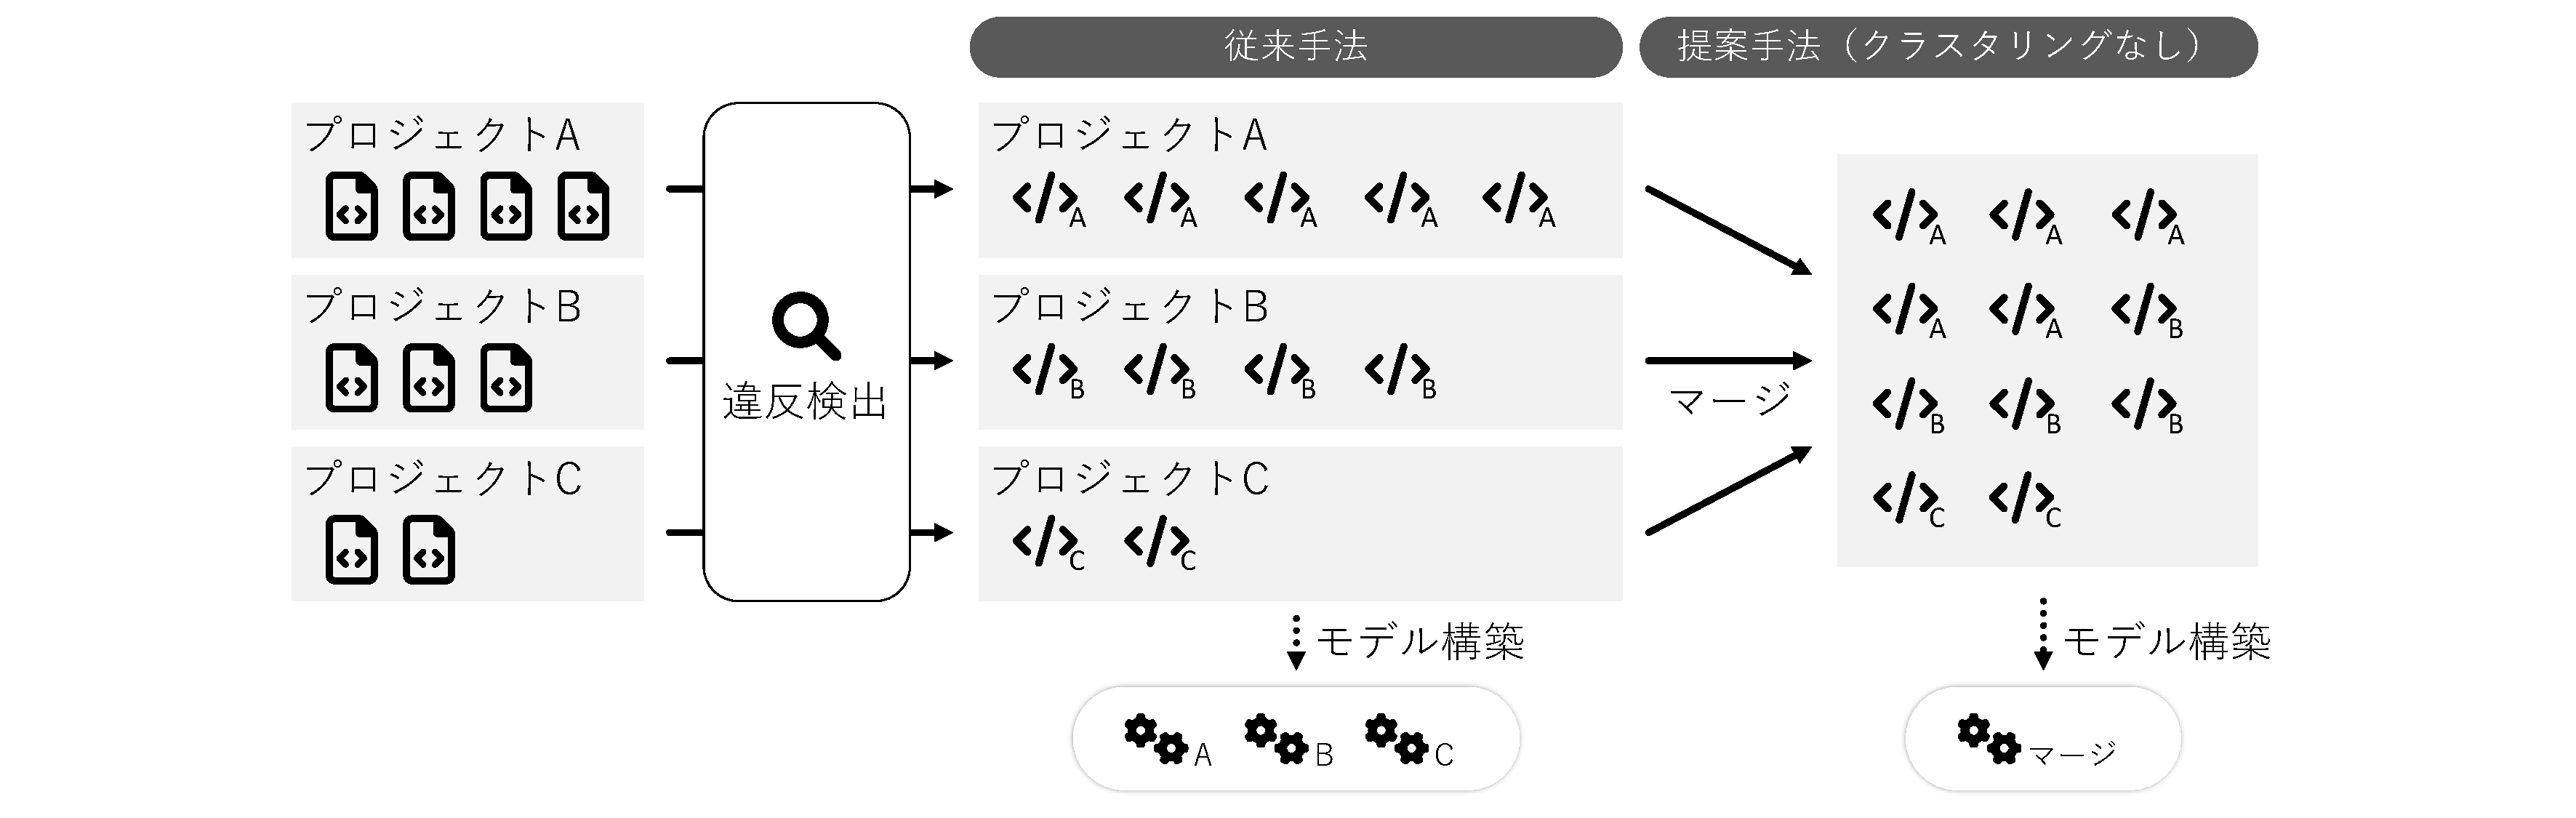
\includegraphics[width=1.0\linewidth]{Kameoka_fig/kameoka_fig1_bw.pdf}
	\caption{本研究の概略図}
	\label{fig:Teiannsyuhou}
\end{figure*}
%------------

図\ref{fig:Teiannsyuhou}は,本研究の提案手法の概略図を示す.本研究では,規約に違反している箇所を修正するか否かを予測する2つの機械学習モデルを構築する.まず,図の左から,各プロジェクトのソースコードを対象に静的解析を行い,規約違反を含むソースコードの特徴量の計測,および,規約違反の修正有無を計測する.次に,学習データとして各プロジェクトの開発履歴のみを用いて機械学習モデル(従来手法)を構築する.従来手法には,Ruthruffらのコードメトリクスなどを説明変数に用いて,ロジスティック回帰モデルによって修正予測する手法を用いる\cite{JyuraiPre}.続いて,各プロジェクトの開発履歴をすべて統合した学習データを用いた機械学習モデル(提案手法)を構築する.




\subsection{学習データと評価データの収集}

本研究では,2種類の提案手法において構築する機械学習モデルにおいて複数のプロジェクトの開発履歴を統合する.具体的には,各プロジェクトの分析対象期間に発生するコミットのうち,前8割を学習データ,後2割を評価データとし,各プロジェクトにおいて未来のデータを含まないようにするため交差検証を行わない.


%ここで,学習データとテスト用データを交差検証を行わない理由は,データセットには,時系列が存在しており,ランダムに学習データとテストデータを分割した場合,学習データに未来の情報を含んでしまうため,データセットの分割時にシャッフルは行わない.

\subsection{説明変数の計測方法}

%-------------------------
\begin{figure}[t]
	\centering
	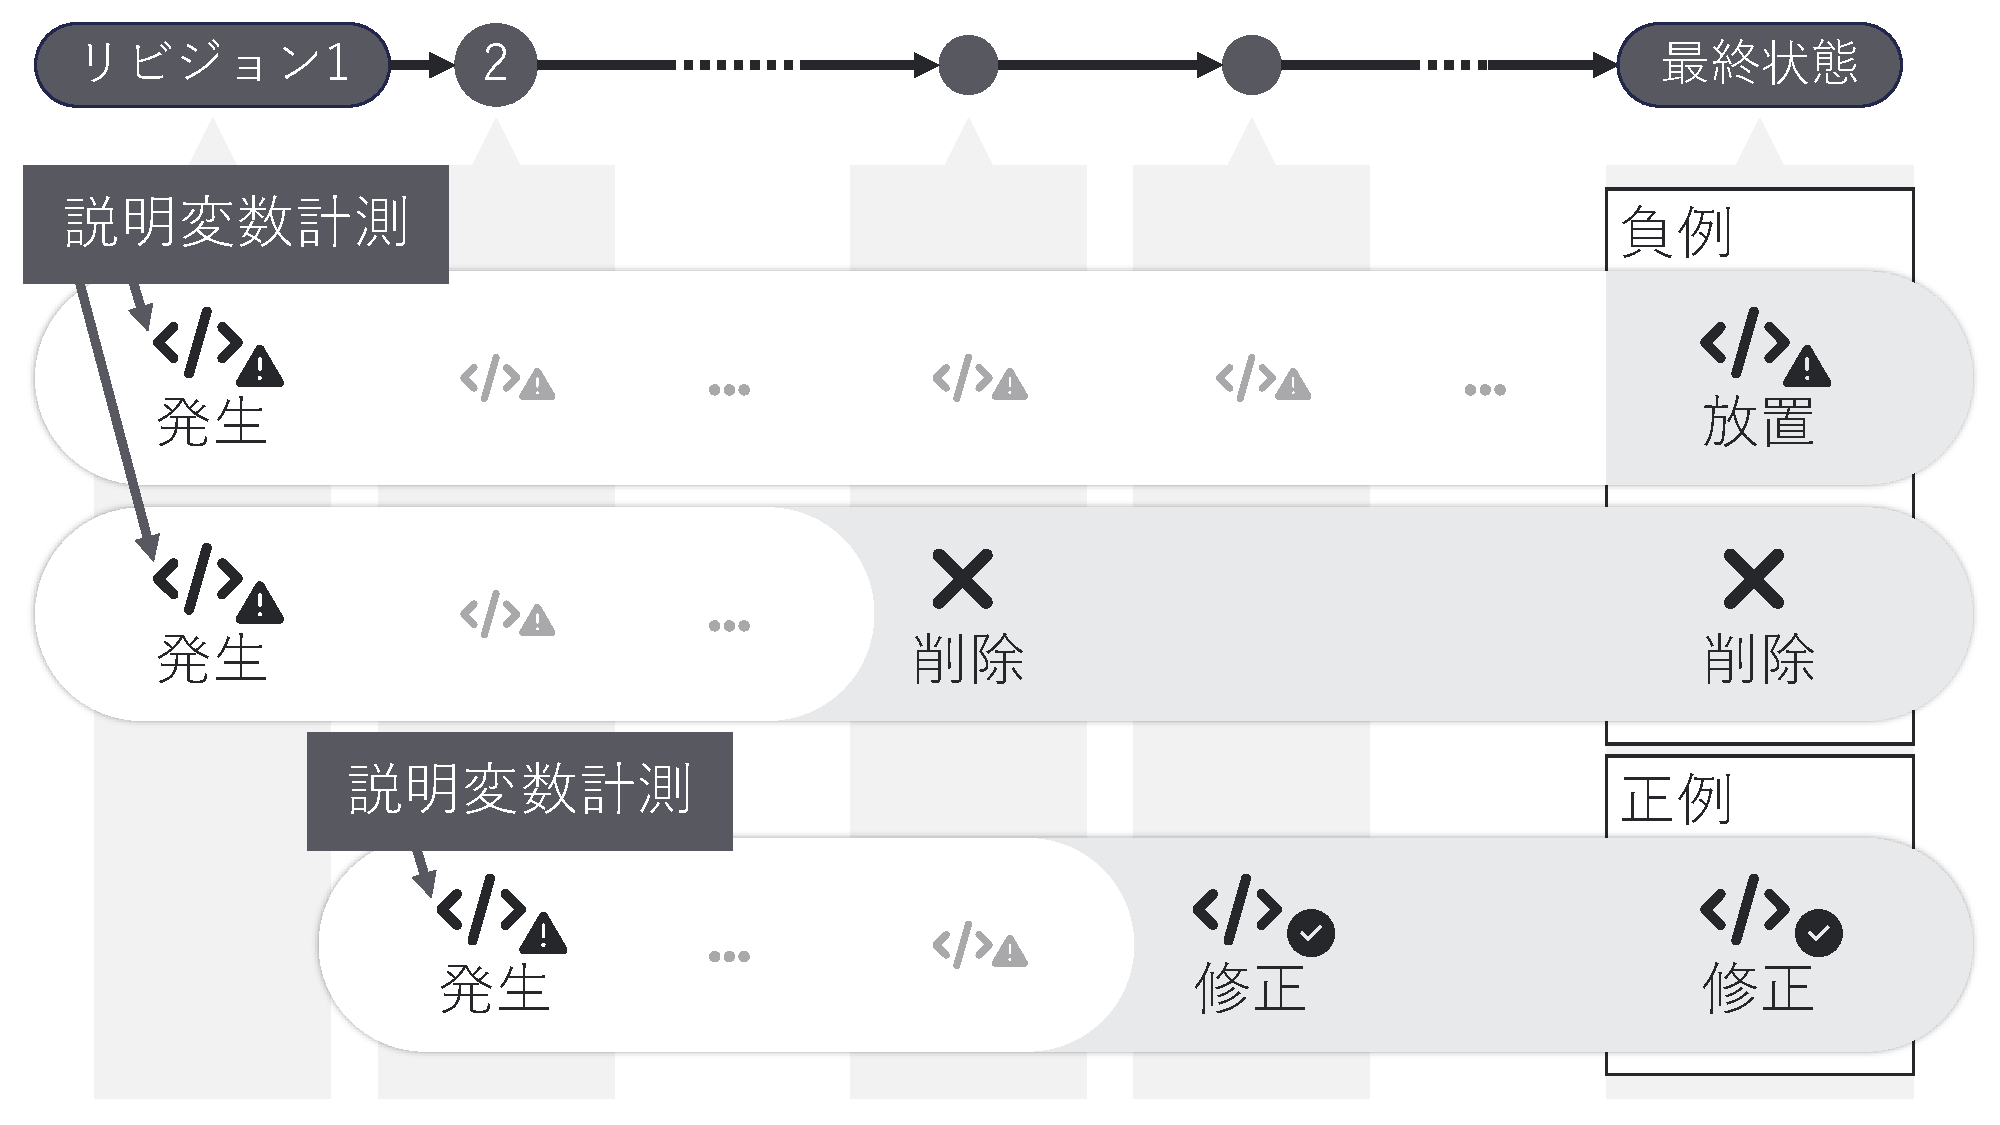
\includegraphics[width=1.0\linewidth]{Kameoka_fig/kameoka_fig2_bw.pdf}
	\caption{説明変数と目的変数の計測方法}
	\label{fig:mokutekihensu}
\end{figure}
%-------------------------

本研究では,分析対象期間中のコミットにおいて変更されたソースコード全てに静的解析ツールを実行する.特定のソースコード断片において初めて規約違反が検出されたコミットを,修正を要するか否かを判定する予測時点とし,説明変数を計測する.

%機械学習モデルの学習,テストに用いる説明変数の計測方法について説明する.まず,説明変数の計測地点について,計測地点はコーディング規約に違反しているコードが生成されたリビジョンである.
図\ref{fig:mokutekihensu}は,説明変数と目的変数の計測事例を示す.この例では,コーディング規約への違反が3箇所で検出され,上2つはリビジョン1で発生し,下の1つはリビジョン2で発生しており,それぞれのリビジョンにおいて説明変数を計測する.ここで説明変数を違反の発生地点で計測する理由は,ファイルの編集箇所で毎回計測を行うと,説明変数の内容は異なるが同じ違反個所に対して複数回学習することとなるので,学習地点では知り得ない未来の情報を学習させないためである.

説明変数の計測地点において,コーディング規約に違反するコード断片を含むソースコードファイルの関数,クラス,モジュールに対して特徴量をテクマトリックス株式会社が開発する静的解析ツールUnderstand\footnote{Understand: \url{https://www.techmatrix.co.jp/product/understand/}}を用いて計測する.説明変数は,ソースコードの特徴量であるコード行数,コメント行数,循環的複雑度,ネストの深さの最大値など含むソースコードに関する特徴量43種類に,コーディング規約の違反検出時に得られる違反箇所のコード行数1種類,規約違反IDをOne-hotベクトル化した1種類の,合計45種類の特徴量を使用する.

\subsection{目的変数の計測方法}

本研究では,分析対象期間中に修正されるか否かを目的変数とする.分析対象期間中に修正された規約違反のコード断片と修正されないままの規約違反含むコード断片は表\ref{tab:pos_neg}に示すように正例と負例の2クラスに分類する.
%図\ref{fig:mokutekihensu}の例を,本分類に従うと上2つは負例,下1つは正例となる.

%----------------------
\begin{table}[t]
    \centering
    \caption{正例と負例の分類}
    \label{tab:pos_neg}
    \scalebox{0.75}{
    \begin{tabular}{l|l}
         \hline
            分類 & 説明\\ \hline
            負例 & コーディング規約の違反が放置されているコード断片\\
            負例 & コーディング規約に違反していたコード断片が削除された\\
            正例 & コーディング規約に違反していたコード断片が修正された\\
         \hline
    \end{tabular}
    }
\end{table}

\subsection{機械学習モデルの構築と評価}

予測モデルの構築には,Ruthruffらの従来研究と同様にロジスティック回帰モデルを用いる\cite{JyuraiPre}.本研究で取り扱うコーディング規約に違反しているコード断片は,修正されないままのコード断片が多数含まれる不均衡なデータとなっている.そのため,ロジスティック回帰分析にはPythonパッケージであるsklearnのlinear\_model.LogisticRegression\footnote{https://scikit-learn.org/stable/modules/generat-\\ed/sklearn.linear\_model.LogisticRegression.html}を使用し,パッケージのオプションclass\_weightsを使用することで2クラスデータの分類に重み付けし,不均衡による問題に対処する.
% また,ロジスティック回帰モデルの学習を行う際にイテレーションの最大値を10,000回に設定する.

予測モデルの予測性能を評価する指標としては,従来研究で用いられている適合率,再現率,F1値を使用する.

%%%%%%%%%%%%%%%%%%%%%%%%%%%%%%%%%%%%%%
\section{評価実験}\label{sec:result}
%%%%%%%%%%%%%%%%%%%%%%%%%%%%%%%%%%%%%%

\subsection{データセット}
%------------
\begin{table*}[t]
    \centering
    \caption{分析対象プロジェクトの統計量(総違反数で昇順に記載)}
    \label{datasetTB}
    \scalebox{1.0}{
    \begin{tabular}{l|r|r|r|r|r}
         \hline
         \multirow{2}{*}{プロジェクト名} & \multirow{2}{*}{対象リビジョン数} & \multicolumn{1}{c|}{違反修正数} & \multicolumn{1}{c|}{違反放置数}& \multicolumn{1}{c|}{\multirow{2}{*}{総違反数}} & \multicolumn{1}{c}{\multirow{2}{*}{違反修正率}} \\ 
                      &               &\multicolumn{1}{c|}{(正例)} & \multicolumn{1}{c|}{(負例)} &&\\ \hline
         \hline %
python-bugzilla & 243 & 189 & 183 & 372 & 51\%\\
python-cloudant & 657 & 269 & 1,299 & 1,568 & 17\%\\
pynput & 507 & 431 & 3,595 & 4,026 & 11\%\\
pyscard & 380 & 681 & 2,705 & 3,386 & 20\%\\
howdoi & 593 & 721 & 434 & 1,155 & 62\%\\
hickle & 245 & 920 & 1,293 & 2,213 & 42\%\\
transitions & 496 & 1,182 & 2,620 & 3,802 & 31\%\\
OWSLib & 422 & 1,547 & 3,080 & 4,627 & 33\%\\
schema\_salad & 564 & 1,990 & 3,009 & 4,999 & 40\%\\
schematics & 524 & 6,950 & 4,829 & 11,779 & 59\%\\
         \hline
    \end{tabular}
    }
\end{table*}
%------------

%--------------------
\begin{table*}[t]
    \centering
    \caption{予測結果}
    \label{PrevPrediction}
    \begin{tabular}{l|ccc|ccc}
         \hline
         \multirow{2}{*}{プロジェクト名}&\multicolumn{3}{c|}{\multirow{1}{*}{従来手法}} & \multicolumn{3}{c}{提案手法}\\
          \cline{2-7}
          & 適合率 & 再現率 & F1値 & 適合率 & 再現率 & F1値\\ \hline
         \hline %
            python-bugzilla & 0.54 & 0.13 & 0.21 & \textbf{\underline{0.69}} & \textbf{\underline{0.64}} & \textbf{\underline{0.67}}\\
            python-cloudant & \textbf{\underline{0.77}} & \textbf{\underline{0.81}} & \textbf{\underline{0.79}} & 0.17 & 0.17 & 0.17\\
            pynput & 0.41 & \textbf{\underline{0.94}} & \textbf{\underline{0.58}} & \textbf{\underline{0.42}} & 0.71 & 0.53\\
            pyscard & \textbf{\underline{0.29}} & \textbf{\underline{0.91}} & \textbf{\underline{0.44}} & 0.18 & 0.89 & 0.30\\
            howdoi & 0.92 & \textbf{\underline{0.96}} & \textbf{\underline{0.94}} & \textbf{\underline{0.93}} & 0.59 & 0.72\\
            hickle & 0.33 & \textbf{\underline{0.73}} & 0.45 & \textbf{\underline{0.36}} & 0.66 & \textbf{\underline{0.47}}\\
            transitions & \textbf{\underline{0.80}} & \textbf{\underline{0.87}} & \textbf{\underline{0.83}} & 0.68 & 0.50 & 0.57\\
            OWSLib & \textbf{\underline{0.84}} & 0.86 & \textbf{\underline{0.85}} & 0.76 & \textbf{\underline{0.92}} & 0.83\\
            schema\_salad & \textbf{\underline{0.52}} & \textbf{\underline{0.66}} & \textbf{\underline{0.58}} & 0.21 & 0.52 & 0.30\\
            schematics & \textbf{\underline{0.30}} & 0.79 & \textbf{\underline{0.44}} & 0.26 & \textbf{\underline{0.94}} & 0.41\\
    \hline
    \end{tabular}
\end{table*}
%--------------------


%--------------------------
%---------------------

本研究ではケーススタディとして,Libraries.io\footnote{Libraries.io: \url{https://libraries.io/}}からPython言語で実装され,静的解析ツールPylintを開発に使用しているプロジェクトを対象とする.当該プロジェクトの中でstar数が上位の100プロジェクトから,コーディング規約違反の修正割合が高い10プロジェクト
% (transitions, schematics, schema\_salad, python-bugzilla, python-cloudant, pyscard, pynput, OWSLib, howdoi, hickle)
を対象とする.すべてのプロジェクトがGitHubによってソフトウェア,および開発履歴を公開している.本研究では,各分析対象プロジェクトにおいて,2018年12月から1,000日間のコミット履歴を分析対象とする.プロジェクト内に含まれるPythonファイルは,テスト用などのファイルの用途は考慮しない.表\ref{datasetTB}は,各プロジェクトに関する開発履歴の統計量を(総違反数で照準に記載)示す.本研究では,コーディング規約違反の修正割合が高いプロジェクトを選定しているが,修正割合はプロジェクトによって大きく異なる.

\subsection{結果}

本研究では,学習データに評価対象とは異なるプロジェクトの開発履歴も使用することにより,違反回数の少ない規約であったとしても特定するモデルを構築する.本手法の有効性を評価するために2種類のモデルを構築し,比較する.
\begin{itemize}
\item \textbf{従来手法}:Ruthruffらの手法\cite{JyuraiPre}をもとにした評価対象プロジェクトと同じプロジェクトの開発履歴を学習するモデル
\item \textbf{本手法}:評価対象プロジェクトを含めた10プロジェクトの開発履歴を学習するモデル
\end{itemize}

表\ref{PrevPrediction}は,従来手法,提案手法により構築した予測モデルの結果を示す.各プロジェクトにおいて3つの手法の中で最も予測性能の高い手法は太字と下線で示す.

\noindent\textbf{知見: 全体的に複数プロジェクトの開発履歴を学習した予測モデルの性能は,評価対象とするプロジェクトの過去の開発履歴のみを学習した予測モデルよりも予測精度が低い.}

各プロジェクトのF1値に着目すると,8プロジェクトでは従来手法が提案手法のF1値を上回った.2プロジェクト(python-bugzilla,hickle)においては従来手法よりも提案手法のほうが予測性能が高く,複数のプロジェクトを使用したとしても精度が下がらないケースがあることを確認した.このことから,提案手法が有効に働く場合があることがわかる.


\section{考察}\label{sec:consideration}
提案手法を用いて複数プロジェクト間でコーディング規約違反の修正予測を行った結果,本研究で使用した10プロジェクトでは全体的な学習データ数が非常に少ない場合,予測精度が向上することが明らかとなった.
% 提案手法として複数プロジェクトの開発履歴を学習に使用することによって,次の特定の状況下において予測精度が向上することが明らかとなった.
% \todo{この条件下でも精度上がらない,維持しない場合があるかは要確認}

% \begin{itemize}
%     \item 全体的な学習データ数が少ない場合
%     \item 修正される(正例)の割合が非常に低い場合
% \end{itemize}

従来手法は,学習データ不足のため予測性能が低いという課題があり,python-bugzillaプロジェクトでは本研究における提案手法においてデータの類似性を問わず複数のプロジェクトの開発履歴を学習することにより正例の割合が増加したことが予測性能の向上に寄与したと示唆される.ただし,正例の割合が小さいプロジェクトとして,pynput(正例割合11\%)では予測性能が向上しているが,python-cloudant(正例割合17\%)では提案手法の予測精度が低下している.
% このような結果の理由の一つとして,python-cloudantは,クラスタリング結果がpynputと比較して多くのクラスタに分かれていることが考えられる.多数のクラスタに分かれたことによってプロジェクト特有の修正に関する特徴を学習できず,予測性能の低下につながったと示唆される.

提案手法はデータ数が少ない場合に有効に働くことが示唆されるため,開発履歴の少ないプロジェクトに適した静的解析ツールによる警告のトリアージに用いることができると考えられる.また,本研究では,プロジェクト間の差異などを考慮していないため,これらを考慮した複数プロジェクトを利用するコーディング規約違反修正予測の研究にも役立つと考えられる.


\section{妥当性への脅威}\label{sec:heuristic}
% \subsection{内的妥当性}

提案手法において複数プロジェクトの開発履歴を用いた際,各プロジェクトにおいてデータセットの分割では時系列を考慮しているが,プロジェクト間では時系列の順序を考慮していない.プロジェクト間においても時系列を考慮した学習データを作成することは今後の課題である.

検証に使用した10プロジェクトは,プロジェクト間の差異を考慮せず,テストコードなどソフトウェアの機能を実装しているファイルとは規約違反の修正の慣習が異なるものを含んでいるため,それらを取り除いた場合,異なる結果になる可能性がある.



% \subsection{外的妥当性}

% 本研究ではケーススタディとして10プロジェクト分のデータを学習し予測を行ったが,データセットを拡張することによって正例が増加し予測性能が向上することも示唆されるが,一方で,学習データ増加により各クラスタで作成したモデルが汎化することも考えられる.今後は,プロジェクト数,クラスタ数の適性についても検討する.


\section{おわりに}\label{sec:end}
本研究では,静的解析ツールによって大量に検出されるコーディング規約に違反しているコード断片の中から,優先して修正すべき違反の予測を,複数プロジェクトのデータを結合することによる予測精度への影響を分析した.検証の結果,予測精度だけを見れば,単一プロジェクトのデータだけを用いて学習するほうが予測に効果的であった.今後は,複数プロジェクトを学習することによる予測結果の違いについて詳細に分析し,コーディング規約に違反しているコード断片の修正予測への影響を明らかにする.

%\textbf{謝辞}\

%\textbf{ありがとうございます.}

% 本フォーマットの基になったスタイルファイルを作成してくださった方々に感謝します.

\bibliographystyle{junsrt}
\bibliography{kameoka}


\end{document}

